% Options for packages loaded elsewhere
\PassOptionsToPackage{unicode}{hyperref}
\PassOptionsToPackage{hyphens}{url}
\PassOptionsToPackage{dvipsnames,svgnames,x11names}{xcolor}
%
\documentclass[
  letterpaper,
  DIV=11,
  numbers=noendperiod]{scrartcl}

\usepackage{amsmath,amssymb}
\usepackage{lmodern}
\usepackage{iftex}
\ifPDFTeX
  \usepackage[T1]{fontenc}
  \usepackage[utf8]{inputenc}
  \usepackage{textcomp} % provide euro and other symbols
\else % if luatex or xetex
  \usepackage{unicode-math}
  \defaultfontfeatures{Scale=MatchLowercase}
  \defaultfontfeatures[\rmfamily]{Ligatures=TeX,Scale=1}
\fi
% Use upquote if available, for straight quotes in verbatim environments
\IfFileExists{upquote.sty}{\usepackage{upquote}}{}
\IfFileExists{microtype.sty}{% use microtype if available
  \usepackage[]{microtype}
  \UseMicrotypeSet[protrusion]{basicmath} % disable protrusion for tt fonts
}{}
\makeatletter
\@ifundefined{KOMAClassName}{% if non-KOMA class
  \IfFileExists{parskip.sty}{%
    \usepackage{parskip}
  }{% else
    \setlength{\parindent}{0pt}
    \setlength{\parskip}{6pt plus 2pt minus 1pt}}
}{% if KOMA class
  \KOMAoptions{parskip=half}}
\makeatother
\usepackage{xcolor}
\setlength{\emergencystretch}{3em} % prevent overfull lines
\setcounter{secnumdepth}{-\maxdimen} % remove section numbering
% Make \paragraph and \subparagraph free-standing
\ifx\paragraph\undefined\else
  \let\oldparagraph\paragraph
  \renewcommand{\paragraph}[1]{\oldparagraph{#1}\mbox{}}
\fi
\ifx\subparagraph\undefined\else
  \let\oldsubparagraph\subparagraph
  \renewcommand{\subparagraph}[1]{\oldsubparagraph{#1}\mbox{}}
\fi


\providecommand{\tightlist}{%
  \setlength{\itemsep}{0pt}\setlength{\parskip}{0pt}}\usepackage{longtable,booktabs,array}
\usepackage{calc} % for calculating minipage widths
% Correct order of tables after \paragraph or \subparagraph
\usepackage{etoolbox}
\makeatletter
\patchcmd\longtable{\par}{\if@noskipsec\mbox{}\fi\par}{}{}
\makeatother
% Allow footnotes in longtable head/foot
\IfFileExists{footnotehyper.sty}{\usepackage{footnotehyper}}{\usepackage{footnote}}
\makesavenoteenv{longtable}
\usepackage{graphicx}
\makeatletter
\def\maxwidth{\ifdim\Gin@nat@width>\linewidth\linewidth\else\Gin@nat@width\fi}
\def\maxheight{\ifdim\Gin@nat@height>\textheight\textheight\else\Gin@nat@height\fi}
\makeatother
% Scale images if necessary, so that they will not overflow the page
% margins by default, and it is still possible to overwrite the defaults
% using explicit options in \includegraphics[width, height, ...]{}
\setkeys{Gin}{width=\maxwidth,height=\maxheight,keepaspectratio}
% Set default figure placement to htbp
\makeatletter
\def\fps@figure{htbp}
\makeatother

\usepackage{booktabs}
\usepackage{longtable}
\usepackage{array}
\usepackage{multirow}
\usepackage{wrapfig}
\usepackage{float}
\usepackage{colortbl}
\usepackage{pdflscape}
\usepackage{tabu}
\usepackage{threeparttable}
\usepackage{threeparttablex}
\usepackage[normalem]{ulem}
\usepackage{makecell}
\usepackage{xcolor}
\usepackage[auth-lg]{authblk}
\KOMAoption{captions}{tableheading}
\makeatletter
\makeatother
\makeatletter
\makeatother
\makeatletter
\@ifpackageloaded{caption}{}{\usepackage{caption}}
\AtBeginDocument{%
\ifdefined\contentsname
  \renewcommand*\contentsname{Table of contents}
\else
  \newcommand\contentsname{Table of contents}
\fi
\ifdefined\listfigurename
  \renewcommand*\listfigurename{List of Figures}
\else
  \newcommand\listfigurename{List of Figures}
\fi
\ifdefined\listtablename
  \renewcommand*\listtablename{List of Tables}
\else
  \newcommand\listtablename{List of Tables}
\fi
\ifdefined\figurename
  \renewcommand*\figurename{Figure}
\else
  \newcommand\figurename{Figure}
\fi
\ifdefined\tablename
  \renewcommand*\tablename{Table}
\else
  \newcommand\tablename{Table}
\fi
}
\@ifpackageloaded{float}{}{\usepackage{float}}
\floatstyle{ruled}
\@ifundefined{c@chapter}{\newfloat{codelisting}{h}{lop}}{\newfloat{codelisting}{h}{lop}[chapter]}
\floatname{codelisting}{Listing}
\newcommand*\listoflistings{\listof{codelisting}{List of Listings}}
\makeatother
\makeatletter
\@ifpackageloaded{caption}{}{\usepackage{caption}}
\@ifpackageloaded{subcaption}{}{\usepackage{subcaption}}
\makeatother
\makeatletter
\@ifpackageloaded{tcolorbox}{}{\usepackage[many]{tcolorbox}}
\makeatother
\makeatletter
\@ifundefined{shadecolor}{\definecolor{shadecolor}{rgb}{.97, .97, .97}}
\makeatother
\makeatletter
\makeatother
\ifLuaTeX
  \usepackage{selnolig}  % disable illegal ligatures
\fi
\IfFileExists{bookmark.sty}{\usepackage{bookmark}}{\usepackage{hyperref}}
\IfFileExists{xurl.sty}{\usepackage{xurl}}{} % add URL line breaks if available
\urlstyle{same} % disable monospaced font for URLs
\hypersetup{
  pdftitle={Trabalho Prático 1},
  pdfauthor={Carolina Musso 18/0047850; Gabriela Carneiro de Almeida 18/0120816; Renan Menezes de Araujo},
  colorlinks=true,
  linkcolor={blue},
  filecolor={Maroon},
  citecolor={Blue},
  urlcolor={Blue},
  pdfcreator={LaTeX via pandoc}}

\title{Trabalho Prático 1}
\usepackage{etoolbox}
\makeatletter
\providecommand{\subtitle}[1]{% add subtitle to \maketitle
  \apptocmd{\@title}{\par {\large #1 \par}}{}{}
}
\makeatother
\subtitle{Séries Temporais - 1/2023}
\author{Carolina Musso 18/0047850 \and Gabriela Carneiro de Almeida
18/0120816 \and Renan Menezes de Araujo}
\date{}

\begin{document}
\maketitle
\ifdefined\Shaded\renewenvironment{Shaded}{\begin{tcolorbox}[enhanced, breakable, interior hidden, borderline west={3pt}{0pt}{shadecolor}, frame hidden, boxrule=0pt, sharp corners]}{\end{tcolorbox}}\fi

\hypertarget{introduuxe7uxe3o}{%
\section{Introdução}\label{introduuxe7uxe3o}}

A pesquisa ``Manufacturers' shipments, paper and allied products'' (M3)
fornece dados estatísticos mensais sobre as condições econômicas no
setor de manufatura doméstica (empresas pequenas). A pesquisa mensura a
atividade industrial atual e fornece uma indicação das tendências
futuras desses tipos de negócios.

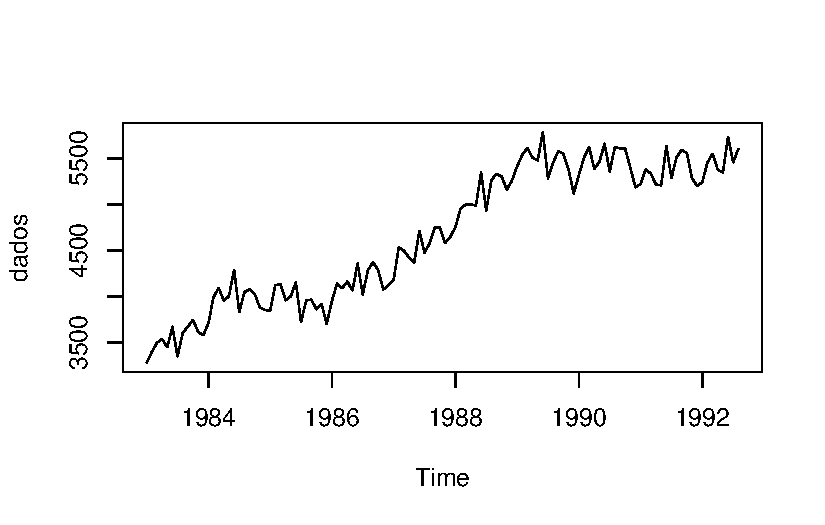
\includegraphics{Trabalhao1_ST_grupo5_files/figure-pdf/unnamed-chunk-2-1.pdf}

\begin{verbatim}
[1] "Manufacturers' shipments, paper and allied products"
\end{verbatim}

\begin{verbatim}
[1] "Passenger cars, from Canada (new), imports (complete units)"
\end{verbatim}

\hypertarget{a.-decomposiuxe7uxe3o-da-suxe9rie-temporal-via-stl-ou-mstl.}{%
\subsection{a. Decomposição da série temporal via STL (ou
MSTL).}\label{a.-decomposiuxe7uxe3o-da-suxe9rie-temporal-via-stl-ou-mstl.}}

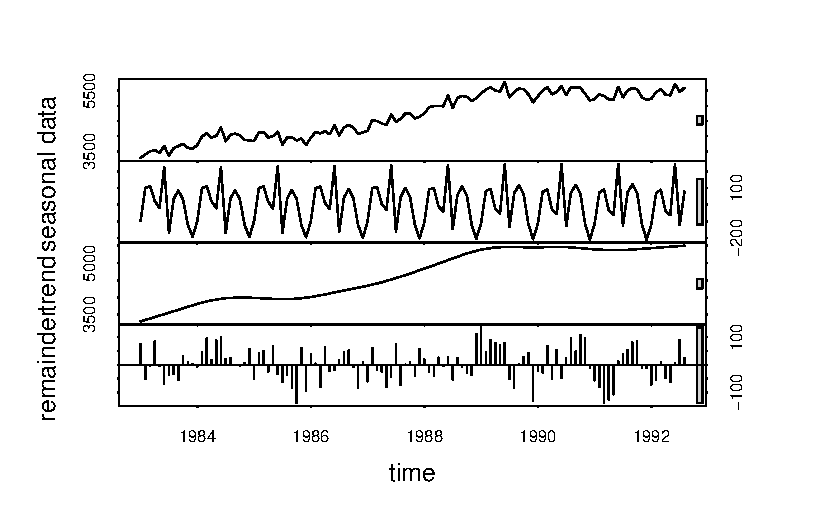
\includegraphics{Trabalhao1_ST_grupo5_files/figure-pdf/unnamed-chunk-3-1.pdf}

Primeiramente a função stl() - ``Seasonal an trending using Loess''- foi
utilizada para decompor a série analisada. Como pode ser observado no
gráfico, há uma tendencia crescente ao longo do tempo analisado e há,
também, uma sazonalidade na série. Porém, a analise de resíduos mostra,
aparentemente, que a decomposição utilizada não foi capaz de decompor a
sazonalidade de uma maneira eficiente, já que ainda há indícios dessa
sazonalidade nos resíduos.

Uma alternativa é utilizar a função de decomposição mstl(), que é uma
versão automatizada. Essa função é capaz de identificar multiplas
sazonalidades.

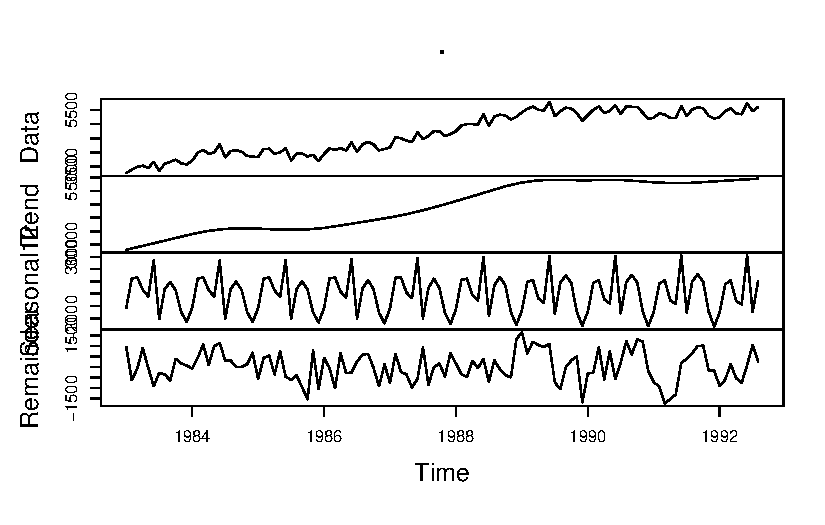
\includegraphics{Trabalhao1_ST_grupo5_files/figure-pdf/unnamed-chunk-4-1.pdf}

O grafico da decomposição MSTL é bem parecido com o gráfico obtido na
decomposição STL, indicando que não há multiplas sazonalidades. Ainda
assim, os resíduos não parecem aleatorizados.

\hypertarget{b.-escolha-um-modelo-arima-adequado-de-forma-manual.}{%
\subsection{b. Escolha um modelo ARIMA adequado de forma
manual.}\label{b.-escolha-um-modelo-arima-adequado-de-forma-manual.}}

\begin{itemize}
\tightlist
\item
  Série ``Manufacturers' shipments, paper and allied products''
\end{itemize}

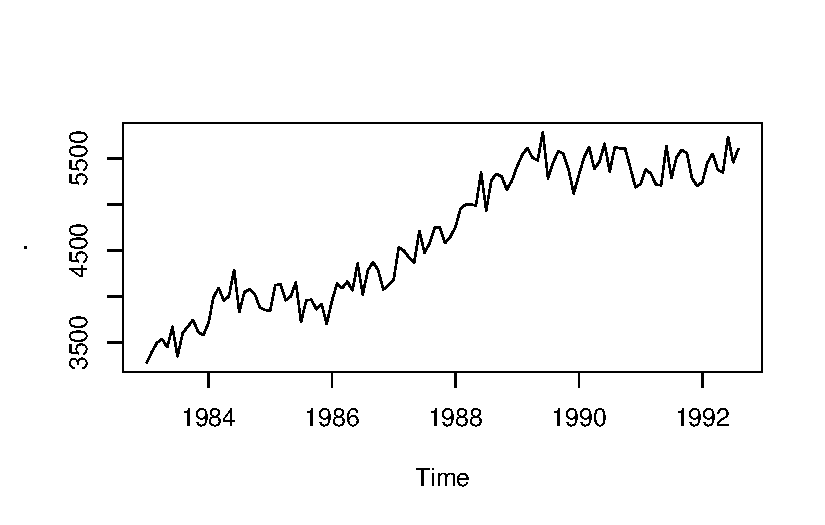
\includegraphics{Trabalhao1_ST_grupo5_files/figure-pdf/unnamed-chunk-5-1.pdf}

\begin{longtable}{cc}
\toprule
Número de diferenciações simples (d) & Número de diferenciações sazonais (D)\\
\midrule
\endfirsthead
\multicolumn{2}{@{}l}{\textit{(continued)}}\\
\toprule
Número de diferenciações simples (d) & Número de diferenciações sazonais (D)\\
\midrule
\endhead

\endfoot
\bottomrule
\endlastfoot
\cellcolor{gray!15}{1} & \cellcolor{gray!15}{1}\\*
\end{longtable}

Conforme observado na tabela acima, a série se torna estacionária com um
diferenciação simples e necessita, também, de uma diferenciação sazonal,
seguindo um modelo

\begin{align*}
  SARIMA (p, 1, q) X (P, 1, Q)
\end{align*}

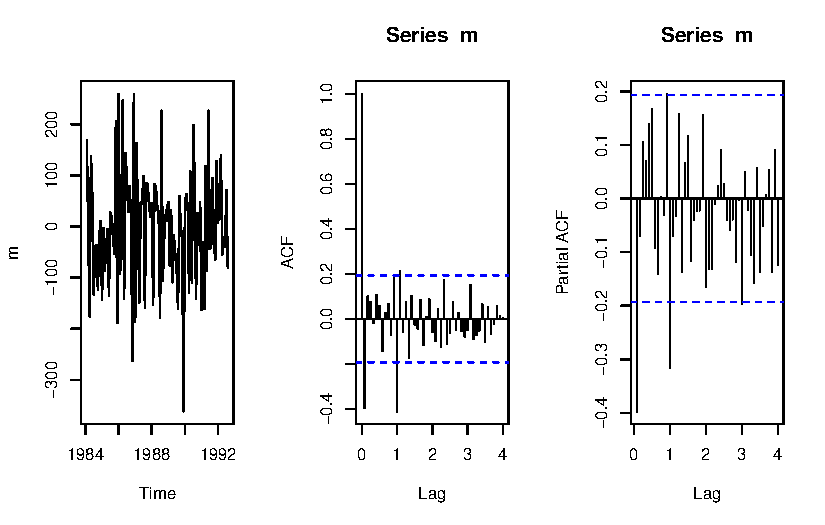
\includegraphics{Trabalhao1_ST_grupo5_files/figure-pdf/unnamed-chunk-7-1.pdf}

\begin{verbatim}
p = 0 , q = 0 , AICc = 1231.865 
p = 0 , q = 1 , AICc = 1151.366 
p = 0 , q = 2 , AICc = 1135.735 
p = 2 , q = 1 , AICc = 1135.723 
\end{verbatim}

Melhor configuração do modelo seria:

\begin{align*}
  SARIMA (2, 1, 1) X (1, 1, 1)
\end{align*}

\begin{verbatim}
Series: dados 
ARIMA(2,1,1)(1,1,1)[12] 

Coefficients:
         ar1     ar2      ma1    sar1     sma1
      0.5266  0.3279  -0.8267  0.0702  -0.8371
s.e.  0.1777  0.0996   0.1549  0.1424   0.1785

sigma^2 = 7297:  log likelihood = -607.97
AIC=1227.95   AICc=1228.82   BIC=1243.76
\end{verbatim}

\hypertarget{c.-anuxe1lise-de-resuxedduos-do-modelo-selecionado.}{%
\subsection{c.~Análise de resíduos do modelo
selecionado.}\label{c.-anuxe1lise-de-resuxedduos-do-modelo-selecionado.}}

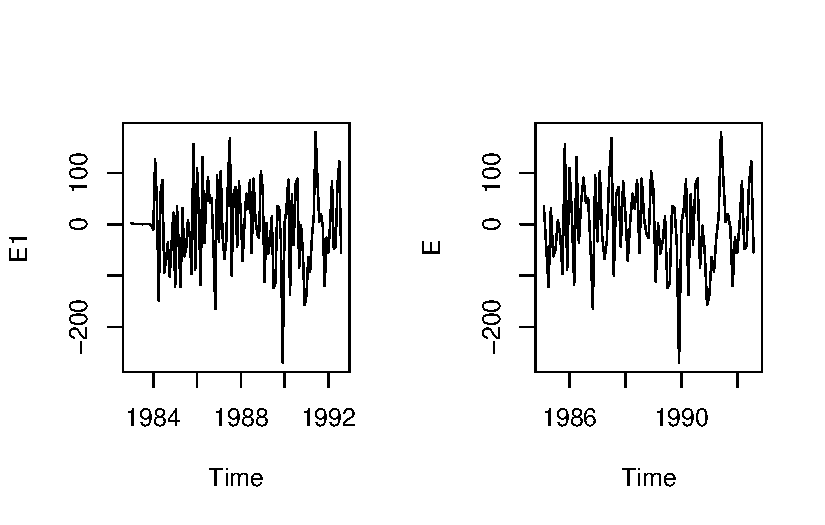
\includegraphics{Trabalhao1_ST_grupo5_files/figure-pdf/unnamed-chunk-10-1.pdf}

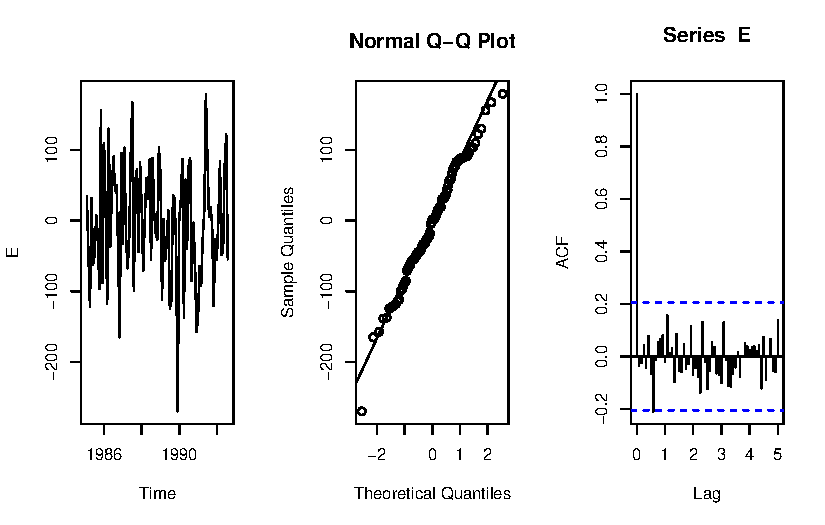
\includegraphics{Trabalhao1_ST_grupo5_files/figure-pdf/unnamed-chunk-11-1.pdf}

\begin{longtable}{ccc}
\toprule
Teste KPSS - estacionariedade & Teste Box-Ljung - independência & Teste Shapiro-Wilk - normalidade\\
\midrule
\endfirsthead
\multicolumn{3}{@{}l}{\textit{(continued)}}\\
\toprule
Teste KPSS - estacionariedade & Teste Box-Ljung - independência & Teste Shapiro-Wilk - normalidade\\
\midrule
\endhead

\endfoot
\bottomrule
\endlastfoot
\cellcolor{gray!15}{0.1} & \cellcolor{gray!15}{0.8065968} & \cellcolor{gray!15}{0.5628871}\\*
\end{longtable}

\hypertarget{d.-comparando-o-modelo-obtido-com-a-funuxe7uxe3o-auto.arima}{%
\subsection{d.~Comparando o modelo obtido com a função
auto.arima}\label{d.-comparando-o-modelo-obtido-com-a-funuxe7uxe3o-auto.arima}}

\begin{verbatim}
Series: dados 
ARIMA(0,1,3)(0,1,1)[12] 

Coefficients:
          ma1     ma2     ma3     sma1
      -0.3485  0.1070  0.1906  -0.7767
s.e.   0.1031  0.0992  0.1180   0.1222

sigma^2 = 7182:  log likelihood = -607.04
AIC=1224.07   AICc=1224.69   BIC=1237.24
\end{verbatim}

\begin{itemize}
\tightlist
\item
  Inclua gráficos e testes estatísticos;
\item
  Comente sobre os resultados;
\end{itemize}

\hypertarget{d.-apresente-a-equauxe7uxe3o-do-modelo-selecionado.}{%
\subsection{d.~Apresente a equação do modelo
selecionado.}\label{d.-apresente-a-equauxe7uxe3o-do-modelo-selecionado.}}

\begin{itemize}
\tightlist
\item
  Utilize a estimava dos parâmetros. Exemplo: o modelo selecionado é um
  AR(1) definido como xt = 0.5xt−1 + εt, t = 1, 2, 3, . . ., em que
  \{εt\} é um processo i.i.d. Normal(0, 3);
\end{itemize}

\hypertarget{e.-no-final-do-relatuxf3rio-inclua-como-um-apuxeandice-o-cuxf3digo-do-r-que-foi-utilizado.}{%
\subsection{e. No final do relatório, inclua como um apêndice o código
do R que foi
utilizado.}\label{e.-no-final-do-relatuxf3rio-inclua-como-um-apuxeandice-o-cuxf3digo-do-r-que-foi-utilizado.}}

\begin{itemize}
\tightlist
\item
  copia r os chucks com echo=T no fim
\end{itemize}



\end{document}
